
\documentclass[journal,12pt,onecolumn]{IEEEtran}
\usepackage{cite}
\usepackage{amsmath,amssymb,amsfonts,amsthm}
\usepackage{algorithmic}
\usepackage{graphicx}
\usepackage{textcomp}
\usepackage{xcolor}
\usepackage{txfonts}
\usepackage{listings}
\usepackage{enumitem}
\usepackage{mathtools}
\usepackage{gensymb}

\usepackage{tkz-euclide} % loads TikZ and tkz-base
\usepackage{listings}

\newtheorem{theorem}{Theorem}[section]
\newtheorem{problem}{Problem}
\newtheorem{proposition}{Proposition}[section]
\newtheorem{lemma}{Lemma}[section]
\newtheorem{corollary}[theorem]{Corollary}
\newtheorem{example}{Example}[section]
\newtheorem{definition}[problem]{Definition}

\theoremstyle{remark}
\newtheorem{rem}{Remark}

\newcommand{\define}{\stackrel{\triangle}{=}}
\newcommand{\system}[1]{\stackrel{#1}{\rightarrow}}

\providecommand{\pr}[1]{\ensuremath{\Pr\left(#1\right)}}
\providecommand{\prt}[2]{\ensuremath{p_{#1}^{\left(#2\right)} }}
\providecommand{\qfunc}[1]{\ensuremath{Q\left(#1\right)}}
\providecommand{\sbrak}[1]{\ensuremath{{}\left[#1\right]}}
\providecommand{\lsbrak}[1]{\ensuremath{{}\left[#1\right.}}
\providecommand{\rsbrak}[1]{\ensuremath{{}\left.#1\right]}}
\providecommand{\brak}[1]{\ensuremath{\left(#1\right)}}
\providecommand{\lbrak}[1]{\ensuremath{\left(#1\right.}}
\providecommand{\rbrak}[1]{\ensuremath{\left.#1\right)}}
\providecommand{\cbrak}[1]{\ensuremath{\left\{#1\right\}}}
\providecommand{\lcbrak}[1]{\ensuremath{\left\{#1\right.}}
\providecommand{\rcbrak}[1]{\ensuremath{\left.#1\right\}}}
\newcommand{\sgn}{\mathop{\mathrm{sgn}}}
\providecommand{\abs}[1]{\left\vert#1\right\vert}
\providecommand{\res}[1]{\Res\displaylimits_{#1}} 
\providecommand{\norm}[1]{\left\lVert#1\right\rVert}

\providecommand{\mean}[1]{E\left[ #1 \right]}
\providecommand{\cond}[2]{#1\middle|#2}
\providecommand{\fourier}{\overset{\mathcal{F}}{ \rightleftharpoons}}
\newenvironment{amatrix}[1]{%
  \left(\begin{array}{@{}*{#1}{c}|c@{}}
}{%
  \end{array}\right)
}

\newcommand{\myvec}[1]{\ensuremath{\begin{pmatrix}#1\end{pmatrix}}}
\newcommand{\mydet}[1]{\ensuremath{\begin{vmatrix}#1\end{vmatrix}}}
\newcommand{\myaugvec}[2]{\ensuremath{\begin{amatrix}{#1}#2\end{amatrix}}}
\providecommand{\rank}{\text{rank}}
\providecommand{\pr}[1]{\ensuremath{\Pr\left(#1\right)}}
\providecommand{\qfunc}[1]{\ensuremath{Q\left(#1\right)}}
\newcommand*{\permcomb}[4][0mu]{{{}^{#3}\mkern#1#2_{#4}}}
\newcommand*{\perm}[1][-3mu]{\permcomb[#1]{P}}
\newcommand*{\comb}[1][-1mu]{\permcomb[#1]{C}}
\providecommand{\gauss}[2]{\mathcal{N}\ensuremath{\left(#1,#2\right)}}
\providecommand{\diff}[2]{\ensuremath{\frac{d{#1}}{d{#2}}}}
\providecommand{\myceil}[1]{\left \lceil #1 \right \rceil }
\newcommand\figref{Fig.~\ref}
\newcommand\tabref{Table~\ref}
\newcommand{\sinc}{\,\text{sinc}\,}
\newcommand{\rect}{\,\text{rect}\,}

\bibliographystyle{IEEEtran}

\bigskip

\renewcommand{\thefigure}{\theenumi}
\renewcommand{\thetable}{\theenumi}

\begin{document}
\title{Discrete Assignment}
\author{Shravya Kantayapalam\\ EE23BTECH11030}
\maketitle

\begin{enumerate}
    \item \textbf{Question 11.9.4.9}:
    Find the sum to $n$ terms of the series whose $n$th term is given by $n^2 + 2^n$?
 \end{enumerate}  
    \textbf{Solution}:
   

\begin{table}[htbp]
    \centering
    \caption{Input Parameters}
    \begin{tabular}{|l|l|l|}
    \hline
    \textbf{Variable} & \textbf{Description} & \textbf{Value} \\
    \hline
    \( x(n) \) & \( n \)-th term of sequence & \( (n^2 + 2^n)u(n) \) \\
    \hline
    \end{tabular}
\end{table}


\begin{align}
y(n) &= (x * u)(n) = \sum_{k=-\infty}^{\infty} x(k) u(n - k)
\end{align}

Given \( (n^2 + 2^n)u(n) \), we have:
\begin{align}
y(n) &= \sum_{k=-\infty}^{\infty} (k^2 + 2^k)u(k)u(n-k)
\end{align}

Applying Z-transform of \( y(n) \) :
\begin{align}
Y(z) &= \sum_{n=0}^{\infty} y(n)z^{-n}
\end{align}

To find \( Y(z) \), we need to use Z-transform pairs:

\begin{align}
n^2 \cdot u(n) &\xleftrightarrow{\text{Z}} \frac{z^{-1}(z^{-1} + 1)}{(1 - z^{-1})^3} \\
2^n \cdot u(n) &\xleftrightarrow{\text{Z}} \frac{1}{1 - 2z^{-1}}
\end{align}

We need to express \( y(n) \) in terms of known Z-transforms to find \( Y(z) \).

Given:

\begin{align}
Y(z) &= \frac{z^{-1}(z^{-1} + 1)}{(1 - z^{-1})^3}  + \frac{2}{1 - 2z^{-1}}
\end{align}

\begin{align}
\frac{z^{-1}(z^{-1} + 1)}{(1 - z^{-1})^3}  &\xleftrightarrow{\mathcal{Z}^{-1}} n^2 u(n) + n u(n) \\
\frac{2}{1 - 2z^{-1}} &\xleftrightarrow{\mathcal{Z}^{-1}} 2 \cdot 2^n u(n)
\end{align}

Therefore, \( y(n) \) is the sum of the above expressions:
\begin{align}
y(n) &= (n^2 + n) u(n) + 2 \cdot 2^n u(n)
\end{align}

\begin{figure}[ht]
    \centering
    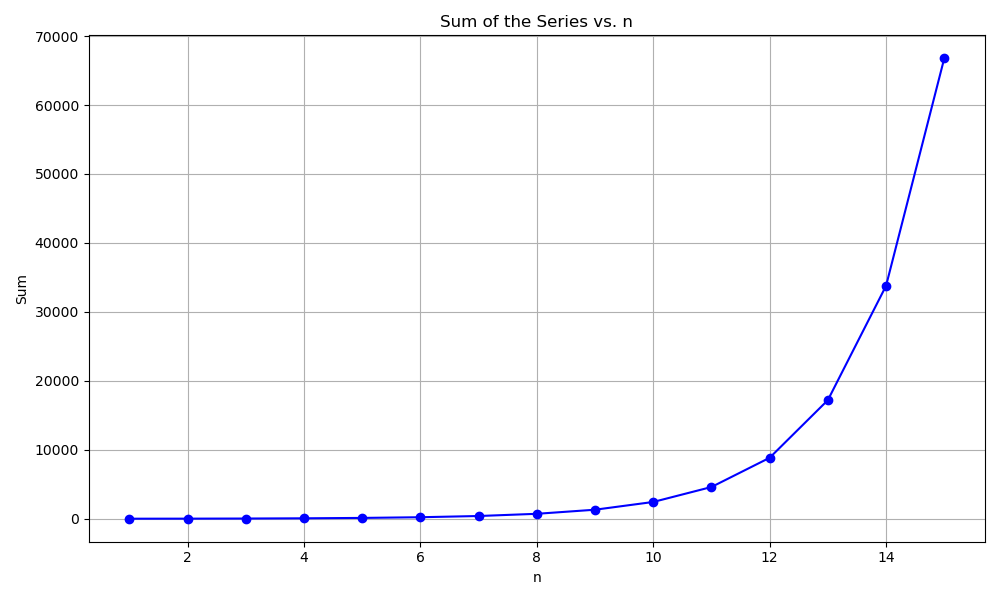
\includegraphics[width=0.5\textwidth]{code/main.png}
    \caption{Graph of $y(n)$ for $n \leq 15$ (Graph beyond $n = 29$ is not shown)}
    \label{fig:example}
\end{figure}

\end{document}

